\documentclass[a4paper,12pt]{article}
\usepackage[slovene]{babel}
\usepackage[utf8]{inputenc}
\usepackage[T1]{fontenc}
\usepackage{lmodern}
\usepackage{amsmath}
\usepackage{amsfonts}
\usepackage{graphicx}

\setlength{\parindent}{0mm}
\pagestyle{empty}

\newcommand{\pojem}[1]{\textsc{#1}}

\newcounter{definicija}
\newenvironment{definicija}
{
   \stepcounter{definicija}
   \begin{flushleft}
   \textbf{Definicija \arabic{definicija}: }
}
{
   \hfill $\square$
   \end{flushleft}
}

\begin{document}

\title{The Prosecutor's Fallacy}
\maketitle

Tožilčeva zmota se pogosto pojavlja v epidemiologiji, vendar jo pogosto neprepoznajo, deloma zato, ker preiskovalci nimajo močne intuicije 
o tem, kaj zmota sploh pomeni. \\
\\
Tožilčeva zmota je dobro znana statistična zmota, ki izhaja iz napačnega razumevanja pogojnih verjetnosti in vprašanj večkratnega testiranja. 
Tu se osredotočamo na vidik pogojne verjetnosti tožilčeve zmote, pri katerei se domneva, da je verjetnost $A$ glede na $B$ enaka verjetnosti 
$B$ glede na $A$:
$$ P(A \lvert B) = P(B \lvert A). $$
Je posledica napačnega razumevanja Bayesovega izreka. \\
\\
Klasičen primer tožilčeve zmote se pojavi, ko tožilec trid, da
\begin{enumerate}
    \item če bi bil obtoženec kriv, bi bila verjetnost dokazov (naprimer ujemanje DNK) velika;
    \item zato mora biti, glede na dokaze, ki so pri roki, verjetnost obtoženčeve krivde velika.
\end{enumerate}
Zmota nastane pri uporabi dokazov in statistike nasploh na sodiščih.
\\
\\
Zmota tožilca se pogosto pojavi v epidemiologiji in javnem zdravju, na primer tveganje za Downov sindrom narašča s starostjo matere, pri čemer je 
tveganje 17 - krat večje pri otrocih, rojenih ženskam, starim 40 let ali več, v primerjavi z otroki, rojenim ženskam, mlajšim od 30 let. Tako lahko 
domnevamo, da je večina žensk, ki rodi otroka z Downovim sindromom, starejših od 40 let; toda raziskava Albermana in Berrya ugotavljata, da se 51\% vseh 
otrok z Downovim sindromom rodi ženskam mlajšim od 30 let, predvsem zato, ker te rojevajo več. \\
Zmota se tudi pogosto pojavi pri razlagi analitičnih rezultatov v epidemiologiji. Na primer, spletna stran Slate.com je objavil izjavo, da je imel eden od 
sedmih otrok s fetanlnim alkoholnim sindromom(FAS) mamo, ki je v prvem tromesečju nosečnosti spila eno do osem pijač na teden; to pomeni: \\
\[ P(\text{mama je spila 1-8 pijač na teden} \lvert FAS) = \frac{1}{7}.\] \\
Toda ta količina nam malo pove o tveganju za FAS glede na določeno raven pitja matere ali \\
\[P(FAS \lvert \text{mama je spila 1-8 pijač na teden}).\]
\\
Zmota se pojavi tudi v epidemiološki literaturi pri zamenjavi občitljivosti (verjetnost pozitivnega testa glede na resnični status bolezni) in pozitivne 
napovedne vrednosti (verjetnost resničnega statusa bolezni glede na pozitiven test).

\section{Vizualizacija Tožilčeve zmote}
Slika 1 prikazuje populacijo 100 moških, starih 50 let, ki se ne zdravijo zaradi hipertenzije in imajo skupni holesterol 235 mg/dl in krvni tlak 120 mmHg. Pričakuje
se, da bo 9\% teh moških (predstavljeno z devetimi črtastimi kvadrati) čez 10 let imelo miokardni infarkt(MI). Ena četrtina moških je kadilcev (predstavljeno s 25 
sivimi kvadrati); približno 16\% naj bi bilemo MI v 10 letih; zato bo $\frac{4}{25}$ kadilcev imelo MI (predstavljeno s črtastimi in sivimi kvadrati). \\
Število kadilcev, ki imajo MI, je očitno enako številu ljudi, ki imajo MI in so kadilci. Toda ali je delež kadilcev, ki imajo MI, enak deležu ljudi z MI, ki so kadilci? Iz 
slike 1 je odogovor očitno ne; verjetnost, da ste kadilec glede na to, da ste imeli MI, torej:
\[ P(\text{MI} \lvert \text{kadilec}) \ne P(\text{kadilec} \lvert \text{MI}), \quad \text{ker}\]
\[ P(\text{MI} \lvert \text{kadilec}) = P(\text{črtasto} \lvert \text{sivo}) = \frac{4}{25} = 0,16 \quad \text{in}\]
\[P(\text{kadilec} \lvert \text{MI}) = P(\text{sivo} \lvert \text{črtasto}) = \frac{4}{9} = 0,44.\]
Vizualno opazimo, da delež sivih kvadratov, ki se prekrivajo s črtastimi kvadrati, ni enak deležu črtastih kvadratov, ki se prekrivajo s sivimi kvadrati. 

\begin{figure}[!ht]
    \centering
    \label{fig:slika1}
    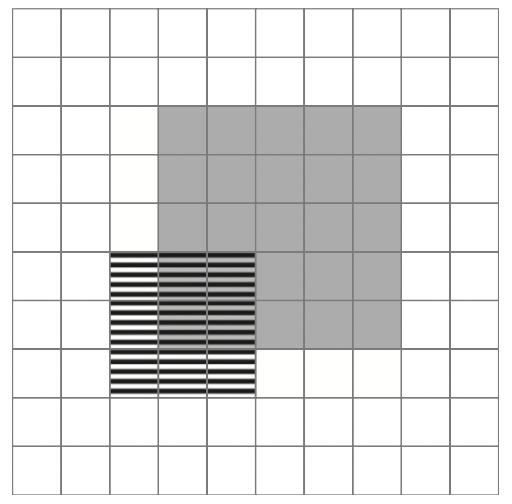
\includegraphics[scale=0.45]{slika1.png}
    \caption{Populacija, predstavljena s 100 kvadrati, z 9 črtastimi, 25 sivimi in 4 črtastimi in sivimi}\vspace{2mm}
 \end{figure}

 Slika 2 prikazuje izjeme pri tožilčevi zmoti, predstavljeni na sliki 1. Sedaj imamo 16 črtastih kvadratov, 16 sivih in 4 pikčaste in sive kvadrate, ker je splošna 
 razširjenost črtastih in sivih kvadratov enaka, je
 \[ P(\text{črtasto} \lvert \text{sivo}) = P(\text{sivo} \lvert \text{črtasto}).\]
Tudi 
\[P(\text{črtasto} \lvert \text{pikčasto}) = P(\text{pikčasto} \lvert \text{črtasto}),\]
saj sta obe verjetnosti enaki $0$. Oboje(podobno velike populacija in populacije brez prekrivanja) je ozka izjema zmote. \\
Po drugi strani pa so črtkani kvadrati na sliki 2 v celoti zajeti v sivih kvadratih; tako je 
\[P(\text{sivo} \lvert \text{črtkano}) = 1, \quad \text{medtem ko je} \quad P(\text{črtkano} \lvert \text{sivo}) = 0,25. \]
Tožilčeva zmota velja, kadar je ena skupina podmnožica druge.

\begin{figure}[!ht]
    \centering
    \label{fig:slika1}
    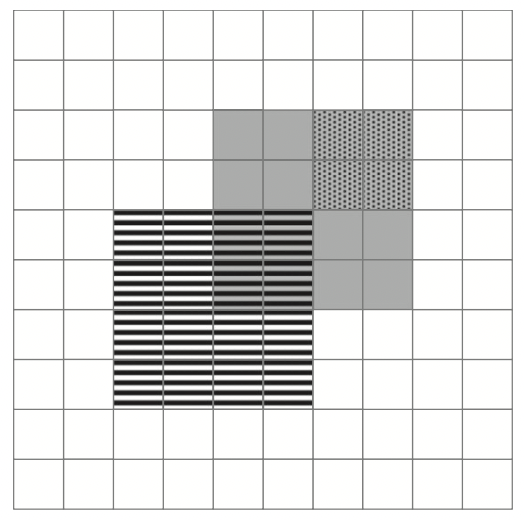
\includegraphics[scale=0.45]{slika2.png}
    \caption{Populacija, predstavljena s 100 kvadrati, z 16 črtastimi, 16 sivimi in 4 pikčastimi in sivimi}\vspace{2mm}
 \end{figure}

\end{document}